\section{Light dark-matter models}\label{sec:1.4}

Kinematics (\cref{sec:1.3}) decides which pairs $(\vect{q}, \omega)$ are open; the interaction with electrons and nuclei decides how often they occur. Model building itself is covered by reviews~\cites[Sect.~III]{lin2019tasi}{kahn2022searches}; we keep only what fixes a rate.

\subsection{Mediators and the Yukawa potential}

Thermal light dark matter needs a mediator with a mass at or below the GeV scale (\cref{sec:1.1}). We take it to be either a massive vector field $A'_\mu$ or a real scalar field $\phi_V$, with mass $m_V$ and couplings $y_\chi$ to dark matter, $y_e$ to electrons and $y_N$ to nucleons. The vector couples to a current of each species and the scalar to a density ($\bar\psi\gamma^\mu\psi$ and $\bar\psi\psi$ in field-theory notation). For slow particles both reduce, at leading order, to the number density~\cite[Eq.~(7)]{knapen2021dark}, and we use only that limit. The interaction Lagrangian densities are then
\begin{equation}
  \mathcal{L}_{\mathrm{int}} = -A'_\mu\bigl(y_\chi J^\mu_\chi + y_e J^\mu_e + y_N J^\mu_N\bigr)
  \quad\text{or}\quad
  \mathcal{L}_{\mathrm{int}} = -\phi_V\bigl(y_\chi \nd_\chi + y_e \nd_e + y_N \nd_N\bigr),
  \label{eq:1.4-Lint}
\end{equation}
where $J^\mu_\chi$, $J^\mu_e$ and $J^\mu_N$ are number currents whose time components are the number densities $\nd_\chi$, $\nd_e$ and $\nd_N$. The spatial components carry a factor of the particle velocity; they lead to velocity-dependent interactions, mentioned at the end of this section, and do not enter the potential below.

The mediator can be treated as a classical field sourced by the particles. A dark-matter particle at rest at the origin is a point source $y_\chi\delta^3(\vect{x})$. For this static source the Euler--Lagrange equation of the vector field reduces to the static Klein--Gordon equation $(-\nabla^2 + m_V^2)A'^0 = y_\chi\delta^3(\vect{x})$ (\cref{eq:C.9-static}). Its solution is $y_\chi$ times the Green's function of \cref{eq:C.9-Gx}, $A'^0(\vect{x}) = y_\chi\,\ee^{-m_V r}/(4\pi r)$ with $r = |\vect{x}|$. By \cref{eq:1.4-Lint}, an electron at $\vect{x}$ has the potential energy $y_e A'^0(\vect{x})$. The dark-matter--electron potential is then
\begin{equation}
  V(\vect{x}) = y_\chi y_e\,\frac{\ee^{-m_V|\vect{x}|}}{4\pi|\vect{x}|},
  \label{eq:1.4-yukawa}
\end{equation}
the Yukawa potential. It has range $1/m_V$ and becomes Coulomb-like as $m_V \to 0$. A scalar mediator leads to the same function with the opposite sign: vector exchange repels sources whose couplings have equal signs, and scalar exchange attracts them (\cref{eq:C.9-U}, where the signs are derived from the field energy). With the Fourier convention of \cref{app:A.3} and \cref{eq:C.9-Gq}, the transform is
\begin{keyresult}[Yukawa potential in momentum space]
\begin{equation}
  \tilde V(\vect{q}) = \int\dd^3x\,\ee^{+\ii\vect{q}\cdot\vect{x}}\,V(\vect{x}) = \frac{y_\chi y_e}{q^2 + m_V^2}.
  \label{eq:1.4-Vq}
\end{equation}
For a scalar mediator the sign is reversed. Since every rate in this book depends on $|\tilde V(\vect{q})|^2$, the sign does not enter.
\end{keyresult}

\noindent Here $\vect{q}$ is the momentum the dark matter transfers to the target (\cref{sec:1.3}). Because $V(\vect{x})$ depends only on the separation, the amplitude for transferring $\vect{q}$ is proportional to $\tilde V(\vect{q})$ (\cref{app:C.9}; derived in \cref{sec:2.2}). \Cref{eq:1.4-Vq} has two limits, which the field calls the heavy- and light-mediator limits. For a heavy mediator, with $m_V$ above every relevant $q$, $\tilde V$ is a constant: a contact interaction. For a light mediator, with $m_V$ below every relevant $q$, $\tilde V \propto 1/q^2$, as in Coulomb scattering. The potential is static because the energy deposited is small: a moving source adds $-\omega^2$ to $q^2 + m_V^2$ in the denominator, and in scattering $\omega \le qv$ with $v \lesssim 3\times10^{-3}$, which keeps the correction below $10^{-5}$ (\cref{app:C.9}).

Which couplings a mediator has depends on the model. A vector coupled to electric charge, the dark photon below, couples to electrons and protons and not to neutrons. A vector coupled to baryon minus lepton number couples to electrons, protons and neutrons with equal magnitude. A scalar that mixes with the Higgs boson couples to each fermion in proportion to its mass, which makes $y_N/y_e$ large~\cite[Sect.~III\,C]{lin2019tasi}. Each mediator is constrained by accelerator, stellar and cosmological data, which bound the products $y_\chi y_e$ and $y_\chi y_N$ that enter rates and the couplings to ordinary matter separately~\cite[Sect.~III\,C]{lin2019tasi}. We will not need these bounds, since the rates below depend on the models only through $\tilde V(\vect{q})$ and the absorption couplings.

\subsection{Reference cross-section and form factor}

Experiments compare models through the reference cross-section $\sigmae$ and the dark-matter form factor $\FDM(q)$, both fixed by $\tilde V(\vect{q})$. The reference momentum is $q_0 = \alpha m_e = \SI{3.73}{keV}$ (\cref{sec:1.3}), the inverse Bohr radius, typical of electrons bound in atoms and solids. We define~\cites[Eqs.~(3) and (4)]{essig2012direct}[Eqs.~(11) and (12)]{knapen2021dark}
\begin{equation}
  \sigmae \equiv \frac{\mu_{\chi e}^2}{\pi}\,|\tilde V(q_0)|^2,
  \qquad
  \FDM(q) \equiv \frac{\tilde V(q)}{\tilde V(q_0)},
  \label{eq:1.4-defs}
\end{equation}
with $\mu_{\chi e}$ the dark-matter--electron reduced mass (\cref{sec:1.3}). Equivalently,
\begin{equation}
  |\tilde V(q)|^2 = \frac{\pi\sigmae}{\mu_{\chi e}^2}\,\FDM(q)^2 ,
  \label{eq:1.4-Vsq}
\end{equation}
the form in which the interaction enters every electron-scattering rate in this book. For the Yukawa potential of \cref{eq:1.4-Vq},
\begin{equation}
  \sigmae = \frac{\mu_{\chi e}^2\, y_\chi^2 y_e^2}{\pi\,(m_V^2 + \alpha^2 m_e^2)^2},
  \qquad
  \FDM(q) = \frac{m_V^2 + \alpha^2 m_e^2}{m_V^2 + q^2},
  \label{eq:1.4-yukawa-sigma}
\end{equation}
in agreement with Ref.~\cite[Eqs.~(11) and (12)]{knapen2021dark}.

Which process does $\sigmae$ describe? For a potential whose transform is a constant $\tilde V$, the first Born approximation yields the free elastic cross-section $\mu_{\chi e}^2|\tilde V|^2/\pi$ (\cref{app:C.9}; derived in \cref{sec:2.2}). It is that cross-section with $\tilde V$ frozen at $q_0$; for a heavy mediator it is the actual cross-section of dark matter on a free electron. For a light mediator, however, it is the cross-section of no process: the free cross-section of a $1/q^2$ potential diverges at small angles, as Rutherford's does, and $\sigmae$ merely normalizes $|\tilde V(q_0)|^2$. In a target the divergence is cut off by the minimum momentum transfer needed to excite it and by screening. Since $\sigmae$ is defined in vacuum, with screening and every other in-medium effect assigned to the target response (\cref{sec:4.4}), a quoted $\sigmae$ means the same thing for every target. Other papers use other reference points and normalizations (\cref{app:A.9}).

Two limits of \cref{eq:1.4-yukawa-sigma} cover most of the literature. A heavy mediator, $m_V$ above both $q_0$ and every momentum transfer that contributes, gives $\FDM = 1$ and $\sigmae = \mu_{\chi e}^2 y_\chi^2 y_e^2/(\pi m_V^4)$. A light mediator, $m_V$ below both, gives $\FDM = (q_0/q)^2$ and $\sigmae = \mu_{\chi e}^2 y_\chi^2 y_e^2/(\pi q_0^4)$. To first order in the small ratio, $\FDM \simeq 1 + (q_0^2 - q^2)/m_V^2$ for the heavy mediator and $\FDM \simeq (q_0/q)^2\,(1 + m_V^2/q_0^2 - m_V^2/q^2)$ for the light one. The momentum transfers that contribute run from $\omega/v_{\mathrm{max}}$, \SI{0.44}{keV} $= 0.12\,q_0$ for the silicon gap, up to $2m_\chi v_{\mathrm{max}}$ (\cref{sec:1.3}).

\begin{limitbox}[Heavy and light mediators][lim:1.4a]
For a mediator of mass $m_V$ and a momentum transfer $q$, the form factor of \cref{eq:1.4-defs} is $\FDM(q) = 1$ when $m_V \gg q, q_0$ (heavy mediator) and $\FDM(q) = (q_0/q)^2$ when $m_V \ll q, q_0$ (light mediator), with $q_0 = \alpha m_e$~\cite[Eq.~(15) and the display above it]{essig2012direct}.
\par\smallskip
{\centering
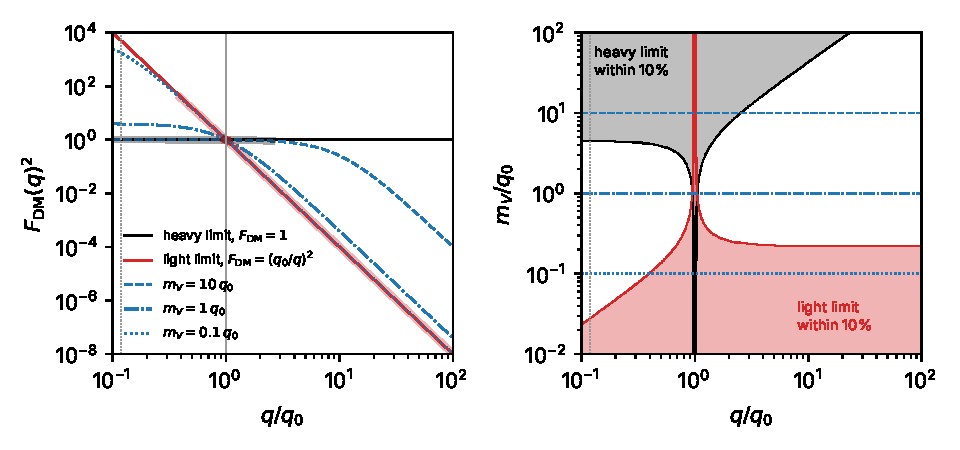
\includegraphics[width=\linewidth]{figures/ch01/fig1_7.pdf}
\captionof{figure}{Squared dark-matter form factor $\FDM(q)^2 = [(m_V^2 + q_0^2)/(m_V^2 + q^2)]^2$~\cite[Eq.~(12)]{knapen2021dark}, with $q_0 = \alpha m_e = \SI{3.73}{keV}$. Left: $\FDM^2$ against $q/q_0$ for $m_V = 10\,q_0$ (dashed), $q_0$ (dash-dotted) and $0.1\,q_0$ (dotted), between the heavy limit $\FDM = 1$ (black) and the light limit $(q_0/q)^4$ (red). A curve is overdrawn in gray or light red where it lies within \SI{10}{\percent} of the heavy or light limit, $|\FDM^2/\text{limit} - 1| \le 0.1$. Right: the same two regions in the plane of $q/q_0$ and $m_V/q_0$; the horizontal lines are the three mediator masses of the left panel. Every curve equals both limits at $q = q_0$ by construction, which produces the narrow vertical strip. Dotted vertical line: $q = 0.12\,q_0$, the smallest momentum transfer that crosses the low-temperature silicon gap. Across $0.12\,q_0 \le q \le q_0$ the heavy limit holds for $m_V \ge 4.5\,q_0 = \SI{17}{keV}$; for all $q \ge 0.12\,q_0$ the light limit holds for $m_V \le 0.028\,q_0 = \SI{0.10}{keV}$.}\label{fig:1-fdm}
\par}
\smallskip
For $m_V$ within a factor of a few of the momentum transfers that the target samples, neither limit holds, and rates must use the full form of \cref{eq:1.4-yukawa-sigma}.
\end{limitbox}

A light mediator weights the rate toward small momentum transfers, by $(q_0/q)^4$, and favors excitations near the kinematic threshold at small $q$, which is also where the target screens most strongly (\cref{sec:4.4}).

\subsection{The dark photon}

The most studied vector mediator is the dark photon: the gauge boson of a new U(1) symmetry under which the dark matter carries charge $y_\chi$ and ordinary matter carries none. It reaches ordinary matter through kinetic mixing, a term $(\zeta/2)F_{\mu\nu}F'^{\mu\nu}$ that couples the photon field strength $F_{\mu\nu}$ to its own, $F'_{\mu\nu}$, with a dimensionless strength $\zeta$~\cite{holdom1986two}. The literature writes $\epsilon$, $\kappa$ or $\chi$ for $\zeta$ (\cref{app:B.2}). Gauge invariance permits the term, and loops of heavy particles charged under both symmetries generate it~\cite{holdom1986two}. The mixing is removed by shifting the photon field, $A_\mu = \tilde A_\mu + \zeta A'_\mu$, which leaves the mass term of $A'_\mu$ unchanged (\cref{eq:C.9-mix,eq:C.9-mixed}).

\begin{keyresult}[Dark-photon couplings]
To first order in $\zeta$, the massive dark photon $A'_\mu$ couples to the dark-matter current with strength $y_\chi$ and to the electromagnetic current $J^\mu_{\mathrm{em}}$ with strength $\zeta e$, through $\mathcal{L} \supset -\zeta e\,A'_\mu J^\mu_{\mathrm{em}} - y_\chi A'_\mu J^\mu_\chi$. Here $e > 0$ is the elementary charge, $e^2 = 4\pi\alpha$ (\cref{app:A.2}), and $J^\mu_{\mathrm{em}}$ counts each particle with its charge in units of $e$. In the notation of \cref{eq:1.4-Lint} the electron coupling is $y_e = -\zeta e$, since the electron charge is $-e$; protons have $+\zeta e$ and neutrons zero. The dark matter stays neutral under the photon.
\end{keyresult}

\noindent Inserting $y_e^2 = 4\pi\alpha\zeta^2$ into \cref{eq:1.4-yukawa-sigma}, we find~\cite[Eq.~(74)]{lin2019tasi}
\begin{equation}
  \sigmae = \frac{4\alpha\,\zeta^2 y_\chi^2\,\mu_{\chi e}^2}{(m_V^2 + \alpha^2 m_e^2)^2}.
  \label{eq:1.4-darkphoton}
\end{equation}
Ref.~\cite[display above Eq.~(15)]{essig2012direct} writes it with $y_\chi^2 = 4\pi\alpha_D$, where $\alpha_D$ is a dark fine-structure constant.

\begin{workedexample}{Reference cross-section of a heavy dark photon}\label{we:1-darkphoton}
We take the thermal-relic benchmark of Ref.~\cite[Sect.~III\,D]{lin2019tasi}: $m_\chi = \SI{10}{MeV}$, $m_V = \SI{30}{MeV}$, $y_\chi = 0.3$ and $\zeta = 10^{-4}$. The reduced mass is $\mu_{\chi e} = m_e m_\chi/(m_e + m_\chi) = (0.511 \times 10/10.511)\,\si{MeV} = \SI{0.486}{MeV}$, so $\mu_{\chi e}^2 = \SI{0.236}{MeV^2}$. The maximum momentum transfer is $2m_\chi v_{\mathrm{max}} = \SI{0.053}{MeV}$, smaller than $m_V$ by a factor of 570: the mediator is heavy, $\FDM = 1$, and $\alpha^2 m_e^2/m_V^2 = 1.5\times10^{-8}$ can be dropped in \cref{eq:1.4-darkphoton}. With $4\alpha = 0.0292$, $\zeta^2 = 10^{-8}$ and $y_\chi^2 = 0.09$,
\begin{equation*}
  \begin{aligned}
  \sigmae &= \frac{4\alpha\,\zeta^2 y_\chi^2\,\mu_{\chi e}^2}{m_V^4}
  = \frac{0.0292 \times 10^{-8} \times 0.09 \times \SI{0.236}{MeV^2}}{(\SI{30}{MeV})^4} \\
  &= \frac{\SI{6.21e-12}{MeV^2}}{\SI{8.10e5}{MeV^4}} = \SI{7.67e-18}{MeV^{-2}}
  \end{aligned}.
\end{equation*}
With $(\hbar c)^2 = \SI{3.894e-22}{MeV^2.cm^2}$ this is $\sigmae = \SI{3.0e-39}{cm^2}$. Ref.~\cite[Sect.~III\,D]{lin2019tasi} quotes about \SI{e-37}{cm^2} for both of its benchmarks, although its own Eq.~(74) leads to the value found here for this one. At fixed couplings $\sigmae$ scales as $m_V^{-4}$, and for $m_\chi \gg m_e$ it hardly depends on $m_\chi$, because $\mu_{\chi e} \to m_e$.
\end{workedexample}

Freeze-out and freeze-in, the two production histories of \cref{sec:1.1}, lead to the heavy- and light-mediator limits of the form factor. Thermal freeze-out through a dark photon needs couplings large enough to deplete the dark matter, which favors a heavy mediator as in \cref{we:1-darkphoton}. Freeze-in, by contrast, needs couplings so feeble that the dark matter never reaches equilibrium; with an ultralight dark photon the rate of scattering on electrons is still observable, because the light-mediator limit enhances small momentum transfers. The freeze-in benchmark of Ref.~\cite[Sect.~III\,D]{lin2019tasi}, $m_\chi = \SI{1}{MeV}$, $m_V = \SI{e-12}{eV}$, $y_\chi = 3\times10^{-6}$ and $\zeta = 10^{-6}$, has $\FDM = (q_0/q)^2$ and, from the light limit of \cref{eq:1.4-darkphoton} with $\mu_{\chi e} = \SI{0.338}{MeV}$, $\sigmae = 4\alpha\zeta^2 y_\chi^2\mu_{\chi e}^2/q_0^4 = \SI{6.1e-38}{cm^2}$.

The field redefinition holds in vacuum. In a medium the photon has a self-energy $\Pi_{\mathrm{em}}$ from the charges it polarizes, and the medium modifies the mixing. For absorption of a dark photon at rest, with $\omega = m_V$ and $q \to 0$, the effective mixing is $\zeta_{\mathrm{eff}}^2 = \zeta^2 m_V^4/\{[m_V^2 - \Real\Pi_{\mathrm{em}}(m_V)]^2 + [\Imag\Pi_{\mathrm{em}}(m_V)]^2\}$~\cite[Eqs.~(5) and (6), with $\kappa$ for $\zeta$]{hochberg2017absorption}. It is suppressed where $m_V$ lies below the scale of $|\Pi_{\mathrm{em}}|$, which in metals and semiconductors is set by the plasma frequency (\cref{sec:4.3}), and approaches $\zeta$ well above it. For scattering, the same physics is the screening of the dark photon's potential by the target. In the convention of this section, where $\tilde V(\vect{q})$ is the unscreened potential, the screening is a factor $1/|\varepsilon(\vect{q}, \omega)|^2$ inside the target response~\cite[Eqs.~(6) and (8)]{knapen2021dark}, and $\sigmae$ stays a vacuum quantity. The self-energy $\Pi_{\mathrm{em}}$ and the longitudinal dielectric function $\varepsilon(\vect{q}, \omega)$ are material quantities: they are measured optically or computed from first principles, in the random-phase approximation with local fields or in time-dependent density-functional theory (\cref{app:E.6}). \Cref{sec:4.4} treats screening, and \cref{chap:10} the in-medium dark photon.

\subsection{Scattering on nuclei}

A mediator that couples to nucleons with strength $y_N$, the same for protons and neutrons, leads to a dark-matter--nucleon potential of the form of \cref{eq:1.4-Vq} with $y_e \to y_N$. For a heavy mediator the dark-matter--proton cross-section is $\sigma_p = \mu_{\chi p}^2 y_\chi^2 y_N^2/(\pi m_V^4)$~\cite[Eq.~(99)]{lin2019tasi}, the analogue of $\sigmae$, with $\mu_{\chi p}$ the dark-matter--proton reduced mass. A nucleus of mass number $A$ and atomic number $Z$ holds $A$ nucleons within a radius of a few fm. When $q$ is small compared with the inverse nuclear radius, $1/R \approx \SI{57}{MeV}$ for silicon, whose nuclear radius is $R \approx \SI{3.47}{fm}$ (\cref{sec:2.2}), the phase $\ee^{\ii\vect{q}\cdot\vect{x}}$ is the same for every nucleon, and the Fourier transform of the summed potential is $A$ times the single-nucleon transform. The amplitudes add coherently.

Replacing $y_N$ by $Ay_N$ and $\mu_{\chi p}$ by the dark-matter--nucleus reduced mass $\mu_{\chi N}$ in $\sigma_p$ gives
\begin{equation}
  \sigma_N = \sigma_p\left(\frac{\mu_{\chi N}}{\mu_{\chi p}}\right)^2 A^2 ,
  \label{eq:1.4-sigmaN}
\end{equation}
the standard convention for spin-independent scattering~\cites{lewin1996review}[Eq.~(104)]{lin2019tasi}. If protons and neutrons couple differently, $A$ becomes $Z + (A - Z)y_n/y_p$, with $y_p$ and $y_n$ the two couplings~\cite[Eq.~(104)]{lin2019tasi}. Since a dark photon couples only to charge, $A^2$ becomes $Z^2$ for it. For silicon, $A = 28$ and $Z = 14$, with the mean atomic mass of natural silicon, \SI{26.16}{GeV}. \Cref{we:2-coherent} evaluates $\sigma_N/\sigma_p$ for silicon.

At larger $q$ the nuclear form factor $F_{\mathrm{Helm}}(q)$ of \cref{sec:2.2} multiplies the amplitude. For the light dark matter of this book the momentum transfer stays below $2m_\chi v_{\mathrm{max}} \approx \SI{5}{MeV}$ even at $m_\chi = \SI{1}{GeV}$, and the nucleus is always coherent. At $q$ below the inverse size of an atom, the electrons screen the nuclear charge seen by a dark photon; this enters through the target response (\cref{sec:4.4}). In a crystal, however, the nuclei are bound, and at low $q$ the dark matter excites phonons instead of free recoils (\cref{chap:5}).

\subsection{Absorption of bosonic dark matter}

Dark matter lighter than about a keV cannot be a thermal relic (\cref{sec:1.1}), but bosons in this range can be produced non-thermally, for example by misalignment, and behave as a classical field oscillating at their mass~\cite[Sect.~I\,B]{lin2019tasi}. Such a boson $\phi$ of mass $m_\phi$ can be absorbed: it disappears and deposits its whole energy in the target. Bound to the Galaxy, it moves at $v \approx 10^{-3}$ and carries energy $m_\phi(1 + v^2/2) \approx m_\phi$ and momentum $\vect{p}_\phi = m_\phi\vect{v}$. Absorption then deposits
\begin{equation}
  \omega \approx m_\phi, \qquad \vect{q} = \vect{p}_\phi, \qquad |\vect{p}_\phi| \approx m_\phi v \approx 10^{-3}\,\omega .
  \label{eq:1.4-absorption}
\end{equation}
The momentum is much smaller than the energy, the reverse of scattering, where $\omega \le qv$ (\cref{sec:1.3}). Absorption probes the response of the target at $q \to 0$, the regime of optical absorption, at a single energy, $\omega = m_\phi$. Compared to scattering, absorption also reaches lower masses. A scattering particle can deposit at most its kinetic energy, and crossing a gap $\Eg$ needs $m_\chi \ge 2\Eg/v_{\mathrm{max}}^2$ (\cref{sec:1.3}), about \SI{0.3}{MeV} for $\Eg \approx \SI{1}{eV}$; an absorbed boson deposits its rest energy and needs only $m_\phi \ge \Eg$, about \SI{1}{eV}. Below the gap, absorption on phonons extends the reach to $m_\phi$ of tens of meV (\cref{chap:5}).

The standard absorbed bosons are the dark photon, the axion-like particle and the scalar. \Cref{app:C.9} derives the classical-field steps that the dark photon shares with scattering, \cref{chap:2} derives absorption rates from the golden rule, and \cref{chap:8} treats each channel. A dark photon that is itself the dark matter, with $m_V = m_\phi$, couples to $J^\mu_{\mathrm{em}}$ exactly as a photon does with $e$ replaced by $\zeta e$. Its absorption rate is the photon absorption rate times $\zeta_{\mathrm{eff}}^2$. Per unit target mass, the normalization of the event rate $\mathcal{R}$ of \cref{sec:1.5}, it is~\cite[Eq.~(7)]{hochberg2017absorption}
\begin{equation}
  \mathcal{R} = \frac{1}{\rho_T}\,\frac{\rho_\chi}{m_\phi}\,\zeta_{\mathrm{eff}}^2\,\sigma_1(m_\phi),
  \label{eq:1.4-dp-abs}
\end{equation}
with $\rho_\chi$ the local dark-matter density (\cref{sec:1.2}), $\rho_T$ the target mass density and $\sigma_1$ the real part of the optical conductivity (\cref{sec:4.4}), measured or computed at $\omega = m_\phi$. The flux of dark matter does not enter, only its number density $\rho_\chi/m_\phi$: an absorbed field deposits energy at a rate set by its amplitude, whatever its speed.

An axion-like particle (ALP), a light pseudoscalar, couples to electrons through $\mathcal{L} \supset g_{aee}\,\phi\,\bar\psi\ii\gamma^5\psi$~\cite[Eq.~(3)]{mitridate2021dark} and to photons through $\mathcal{L} \supset -\tfrac14 g_{a\gamma\gamma}\,\phi\,F_{\mu\nu}\tilde F^{\mu\nu} = g_{a\gamma\gamma}\,\phi\,\vect{E}\cdot\vect{B}$, with $\tilde F^{\mu\nu}$ the dual field strength~\cite[Eqs.~(2) and (3)]{graham2015experimental}; the subscript $a$ names the ALP. At low energy the electron field $\psi$ reduces to a two-component field $\op\psi$ (the field operator of \cref{sec:2.3}), and the electron coupling becomes~\cite[Eq.~(18) and Table~I]{mitridate2021dark}
\begin{equation}
  \mathcal{L}_{aee} = -\frac{g_{aee}}{2m_e}\,(\nabla\phi)\cdot\bigl(\op\psi^\dagger\boldsymbol{\sigma}\op\psi\bigr)
  + \frac{\ii g_{aee}}{4m_e^2}\,(\partial_t\phi)\,\op\psi^\dagger\boldsymbol{\sigma}\cdot\overleftrightarrow{\nabla}\op\psi ,
  \label{eq:1.4-alp}
\end{equation}
with $\boldsymbol{\sigma}$ the Pauli matrices and $\op\psi^\dagger\overleftrightarrow{\nabla}\op\psi \equiv \op\psi^\dagger(\nabla\op\psi) - (\nabla\op\psi^\dagger)\op\psi$. The first term couples $\nabla\phi$, of size $|\vect{p}_\phi|\phi$, to the electron spin density and is suppressed by $|\vect{p}_\phi|$. The second couples $\partial_t\phi$, of size $m_\phi\phi$, to the electron spin-current. Compared with the first, it trades the dark-matter velocity, typically $10^{-3}$, for the electron velocity $|\nabla|/m_e$, typically $\sim \alpha$ in a solid; as a result it dominates absorption, although it is formally of higher order in $1/m_e$~\cite[Sect.~II]{mitridate2021dark}. When spin--orbit coupling is negligible its rate follows from the optical conductivity, like that of a dark photon~\cite[Table~I]{mitridate2021dark}. The photon coupling contributes to absorption in a solid only in a static magnetic field $\vect{B}_0$: there $\phi$ drives an electric field along $\vect{B}_0$ that oscillates at $m_\phi$, and the ALP is absorbed like a dark photon polarized along $\vect{B}_0$.

A scalar couples through $\mathcal{L} \supset g_{\phi ee}\,\phi\,\bar\psi\psi$~\cite[Eq.~(3)]{mitridate2021dark}, which at low energy becomes~\cite[Eq.~(18) and Table~I]{mitridate2021dark}
\begin{equation}
  \mathcal{L}_{\phi ee} = g_{\phi ee}\,\phi\,\op\psi^\dagger\op\psi + \frac{g_{\phi ee}}{8m_e^2}\,\phi\,\op\psi^\dagger\overleftrightarrow{\nabla}^{2}\op\psi ,
  \label{eq:1.4-scalar}
\end{equation}
where a third term of Ref.~\cite[Eq.~(18)]{mitridate2021dark}, involving the photon field, is omitted because it does not contribute to absorption in an isotropic medium~\cite[Table~I]{mitridate2021dark}, and $\op\psi^\dagger\overleftrightarrow{\nabla}^{2}\op\psi \equiv \op\psi^\dagger(\nabla^2\op\psi) + (\nabla^2\op\psi^\dagger)\op\psi - 2(\nabla\op\psi^\dagger)\cdot(\nabla\op\psi)$. The first term couples to the electron number density, whose matrix elements between different states vanish as $\vect{p}_\phi \to 0$ by charge conservation. The second, a kinetic-energy density, dominates, and its rate is not fixed by the optical conductivity~\cite[Table~I]{mitridate2021dark}. \Cref{tab:1-interactions} collects the interactions of this section.

\begin{table}[t]
  \caption{Interactions of light dark matter used in this book. Each row gives the coupling, the target quantity that sets the rate and the excitation that dominates in a semiconductor. The density response and conductivity are defined in \cref{chap:4}, the spin and kinetic-energy responses in \cref{chap:8}, and phonons in \cref{chap:5}.}
  \label{tab:1-interactions}
  \centering\small
  \begin{tabular}{@{}>{\raggedright\arraybackslash}p{0.22\linewidth}>{\raggedright\arraybackslash}p{0.16\linewidth}>{\raggedright\arraybackslash}p{0.27\linewidth}>{\raggedright\arraybackslash}p{0.25\linewidth}@{}}
    \toprule
    Interaction & Coupling & Target quantity & Dominant excitation \\
    \midrule
    Scattering, heavy mediator & $\sigmae$, $\FDM = 1$ & electron density response at all $q$ & electron--hole pairs \\
    Scattering, light mediator & $\sigmae$, $\FDM = (q_0/q)^2$ & electron density response at small $q$, screened & electron--hole pairs near threshold \\
    Scattering on nuclei & $\sigma_p$, $\sigma_N$ & nuclear density response & phonons; nuclear recoils above the binding scale \\
    Dark-photon absorption & $\zeta$ & optical conductivity at $\omega = m_\phi$ & electron--hole pairs above the gap; optical phonons in polar crystals below it \\
    ALP absorption & $g_{aee}$; $g_{a\gamma\gamma}$ & electron spin-current response; field $\vect{B}_0$ & electron--hole pairs; photons in $\vect{B}_0$ \\
    Scalar absorption & $g_{\phi ee}$ & electron kinetic-energy response & electron--hole pairs \\
    \bottomrule
  \end{tabular}
\end{table}

\subsection{Inelastic dark matter and further interactions}

The dark matter may have two nearly degenerate states, $\chi_1$ and $\chi_2$, split by $\Delta_\chi = m_{\chi_2} - m_{\chi_1}$. This happens, for example, when a small mass term splits one dark-matter particle into two states of slightly different mass, and the mediator couples only across them, so every scattering changes the state~\cite{tuckersmith2001inelastic}; in field-theory language, a Dirac fermion splits into two Majorana states. The potential and $\sigmae$ keep their form; only the kinematics changes, through the term $-\Delta_\chi$ in the energy transfer $\omega_{\vect{q}}$ of \cref{eq:1.3-omegaq}, with the endothermic and exothermic cases of \cref{sec:1.3}.

The mediators of this section lead to the simplest non-relativistic interaction, a spin-independent potential. A general basis of non-relativistic interactions exists, built from $\vect{q}$, the relative velocity and the spins of the dark matter and the target~\cite{fitzpatrick2013effective}; the Yukawa potential is its first, spin-independent operator multiplied by $\FDM(q)$. \Cref{chap:8} treats this basis and the target responses it requires.
